\documentclass[ngerman]{article}
%DIF LATEXDIFF DIFFERENCE FILE
%DIF DEL old-expose.tex   Mon Feb  5 12:28:42 2024
%DIF ADD expose.tex       Mon Feb  5 12:24:36 2024

\usepackage{xcolor}
\usepackage{inconsolata}
\usepackage[T1]{fontenc}
\usepackage{pgffor}
\usepackage{graphicx}
\usepackage{fancyhdr}
\usepackage{hyperref}
\usepackage{tcolorbox}
\usepackage[margin=1.2in]{geometry}
\usepackage[ngerman]{babel} 
\usepackage{bookmark}
\usepackage[sorting=none, autolang=other, backend=biber]{biblatex}
\addbibresource{refs.bib}


\hypersetup{
  colorlinks=true,
  linkcolor=blue,
  filecolor=magenta,
  citecolor=blue,
  urlcolor=blue,
}

\renewcommand*\familydefault{\ttdefault} %% Only if the base font of the document is to be typewriter style

\newcommand{\topic}[1]{\tcbox[on line,arc=4pt,colframe=white,boxrule=0pt,boxsep=0pt,left=4pt,right=4pt,top=3pt,bottom=2pt,colback=gray!30]{#1}}

% Define a custom command for colored boxes around words
\newcommand{\topics}[1]{%
  \linebreak
  \linebreak
  \foreach \word in {#1} {%
    \topic{\word}%
  }%
  \linebreak
}


\title{Exposé für eine Bachelorarbeit}
\author{Max Richter}
%DIF PREAMBLE EXTENSION ADDED BY LATEXDIFF
%DIF UNDERLINE PREAMBLE %DIF PREAMBLE
\RequirePackage[normalem]{ulem} %DIF PREAMBLE
\RequirePackage{color}\definecolor{RED}{rgb}{1,0,0}\definecolor{BLUE}{rgb}{0,0,1} %DIF PREAMBLE
\providecommand{\DIFaddtex}[1]{{\protect\color{blue}\uwave{#1}}} %DIF PREAMBLE
\providecommand{\DIFdeltex}[1]{{\protect\color{red}\sout{#1}}}                      %DIF PREAMBLE
%DIF SAFE PREAMBLE %DIF PREAMBLE
\providecommand{\DIFaddbegin}{} %DIF PREAMBLE
\providecommand{\DIFaddend}{} %DIF PREAMBLE
\providecommand{\DIFdelbegin}{} %DIF PREAMBLE
\providecommand{\DIFdelend}{} %DIF PREAMBLE
\providecommand{\DIFmodbegin}{} %DIF PREAMBLE
\providecommand{\DIFmodend}{} %DIF PREAMBLE
%DIF FLOATSAFE PREAMBLE %DIF PREAMBLE
\providecommand{\DIFaddFL}[1]{\DIFadd{#1}} %DIF PREAMBLE
\providecommand{\DIFdelFL}[1]{\DIFdel{#1}} %DIF PREAMBLE
\providecommand{\DIFaddbeginFL}{} %DIF PREAMBLE
\providecommand{\DIFaddendFL}{} %DIF PREAMBLE
\providecommand{\DIFdelbeginFL}{} %DIF PREAMBLE
\providecommand{\DIFdelendFL}{} %DIF PREAMBLE
%DIF HYPERREF PREAMBLE %DIF PREAMBLE
\providecommand{\DIFadd}[1]{\texorpdfstring{\DIFaddtex{#1}}{#1}} %DIF PREAMBLE
\providecommand{\DIFdel}[1]{\texorpdfstring{\DIFdeltex{#1}}{}} %DIF PREAMBLE
\newcommand{\DIFscaledelfig}{0.5}
%DIF HIGHLIGHTGRAPHICS PREAMBLE %DIF PREAMBLE
\RequirePackage{settobox} %DIF PREAMBLE
\RequirePackage{letltxmacro} %DIF PREAMBLE
\newsavebox{\DIFdelgraphicsbox} %DIF PREAMBLE
\newlength{\DIFdelgraphicswidth} %DIF PREAMBLE
\newlength{\DIFdelgraphicsheight} %DIF PREAMBLE
% store original definition of \includegraphics %DIF PREAMBLE
\LetLtxMacro{\DIFOincludegraphics}{\includegraphics} %DIF PREAMBLE
\newcommand{\DIFaddincludegraphics}[2][]{{\color{blue}\fbox{\DIFOincludegraphics[#1]{#2}}}} %DIF PREAMBLE
\newcommand{\DIFdelincludegraphics}[2][]{% %DIF PREAMBLE
\sbox{\DIFdelgraphicsbox}{\DIFOincludegraphics[#1]{#2}}% %DIF PREAMBLE
\settoboxwidth{\DIFdelgraphicswidth}{\DIFdelgraphicsbox} %DIF PREAMBLE
\settoboxtotalheight{\DIFdelgraphicsheight}{\DIFdelgraphicsbox} %DIF PREAMBLE
\scalebox{\DIFscaledelfig}{% %DIF PREAMBLE
\parbox[b]{\DIFdelgraphicswidth}{\usebox{\DIFdelgraphicsbox}\\[-\baselineskip] \rule{\DIFdelgraphicswidth}{0em}}\llap{\resizebox{\DIFdelgraphicswidth}{\DIFdelgraphicsheight}{% %DIF PREAMBLE
\setlength{\unitlength}{\DIFdelgraphicswidth}% %DIF PREAMBLE
\begin{picture}(1,1)% %DIF PREAMBLE
\thicklines\linethickness{2pt} %DIF PREAMBLE
{\color[rgb]{1,0,0}\put(0,0){\framebox(1,1){}}}% %DIF PREAMBLE
{\color[rgb]{1,0,0}\put(0,0){\line( 1,1){1}}}% %DIF PREAMBLE
{\color[rgb]{1,0,0}\put(0,1){\line(1,-1){1}}}% %DIF PREAMBLE
\end{picture}% %DIF PREAMBLE
}\hspace*{3pt}}} %DIF PREAMBLE
} %DIF PREAMBLE
\LetLtxMacro{\DIFOaddbegin}{\DIFaddbegin} %DIF PREAMBLE
\LetLtxMacro{\DIFOaddend}{\DIFaddend} %DIF PREAMBLE
\LetLtxMacro{\DIFOdelbegin}{\DIFdelbegin} %DIF PREAMBLE
\LetLtxMacro{\DIFOdelend}{\DIFdelend} %DIF PREAMBLE
\DeclareRobustCommand{\DIFaddbegin}{\DIFOaddbegin \let\includegraphics\DIFaddincludegraphics} %DIF PREAMBLE
\DeclareRobustCommand{\DIFaddend}{\DIFOaddend \let\includegraphics\DIFOincludegraphics} %DIF PREAMBLE
\DeclareRobustCommand{\DIFdelbegin}{\DIFOdelbegin \let\includegraphics\DIFdelincludegraphics} %DIF PREAMBLE
\DeclareRobustCommand{\DIFdelend}{\DIFOaddend \let\includegraphics\DIFOincludegraphics} %DIF PREAMBLE
\LetLtxMacro{\DIFOaddbeginFL}{\DIFaddbeginFL} %DIF PREAMBLE
\LetLtxMacro{\DIFOaddendFL}{\DIFaddendFL} %DIF PREAMBLE
\LetLtxMacro{\DIFOdelbeginFL}{\DIFdelbeginFL} %DIF PREAMBLE
\LetLtxMacro{\DIFOdelendFL}{\DIFdelendFL} %DIF PREAMBLE
\DeclareRobustCommand{\DIFaddbeginFL}{\DIFOaddbeginFL \let\includegraphics\DIFaddincludegraphics} %DIF PREAMBLE
\DeclareRobustCommand{\DIFaddendFL}{\DIFOaddendFL \let\includegraphics\DIFOincludegraphics} %DIF PREAMBLE
\DeclareRobustCommand{\DIFdelbeginFL}{\DIFOdelbeginFL \let\includegraphics\DIFdelincludegraphics} %DIF PREAMBLE
\DeclareRobustCommand{\DIFdelendFL}{\DIFOaddendFL \let\includegraphics\DIFOincludegraphics} %DIF PREAMBLE
%DIF COLORLISTINGS PREAMBLE %DIF PREAMBLE
\RequirePackage{listings} %DIF PREAMBLE
\RequirePackage{color} %DIF PREAMBLE
\lstdefinelanguage{DIFcode}{ %DIF PREAMBLE
%DIF DIFCODE_UNDERLINE %DIF PREAMBLE
  moredelim=[il][\color{red}\sout]{\%DIF\ <\ }, %DIF PREAMBLE
  moredelim=[il][\color{blue}\uwave]{\%DIF\ >\ } %DIF PREAMBLE
} %DIF PREAMBLE
\lstdefinestyle{DIFverbatimstyle}{ %DIF PREAMBLE
	language=DIFcode, %DIF PREAMBLE
	basicstyle=\ttfamily, %DIF PREAMBLE
	columns=fullflexible, %DIF PREAMBLE
	keepspaces=true %DIF PREAMBLE
} %DIF PREAMBLE
\lstnewenvironment{DIFverbatim}{\lstset{style=DIFverbatimstyle}}{} %DIF PREAMBLE
\lstnewenvironment{DIFverbatim*}{\lstset{style=DIFverbatimstyle,showspaces=true}}{} %DIF PREAMBLE
%DIF END PREAMBLE EXTENSION ADDED BY LATEXDIFF

\begin{document}

\pagestyle{fancy}
\fancyhead{} % clear all header fields
\fancyhead[RO,LE]{\textbf{WebAssembly-basierte visuelle Programmiersprache}}
\fancyfoot{} % clear all footer fields
\fancyfoot[LE,RO]{\thepage}
\fancyfoot[LO,CE]{\href{https://github.com/jim-fx/bachelor}{github.com/jim-fx/bachelor}}
\fancyfoot[CO,RE]{Max Richter}

\raggedright

\maketitle
\pagebreak

{\LARGE Entwicklung einer performanten WebAssembly-basierten visuellen Programmiersprache}

\section{Problemstellung}
In unserer heutigen digitalisierten Welt spielen Human-Computer Interfaces eine entscheidende Rolle. Hierbei gibt es eine weite Spanne von Komplexität, von einfach zu bedienenden grafischen Benutzeroberflächen bis zu komplexen Programmiersprachen. Meiner Meinung nach bieten visuelle Programmiersprachen einen guten Mittelweg für programmierunerfahrenen Nutzer*innen.
Sie vereinen die Benutzerfreundlichkeit grafischer Interfaces mit der Komplexität und Flexibilität textbasierter Programmiersprachen. 
\linebreak
\linebreak
In dieser Bachelorarbeit werde ich eine node-basierte visuelle Programmiersprache entwickeln bei der die einzelnen Nodes WebAssembly Module sind. Diese Programmiersprache soll es Nutzer*innen ermöglichen, eigene Nodes für unterschiedlichste Anwendungsfälle zu entwickeln und miteinander zu teilen.
\begin{figure}[h]
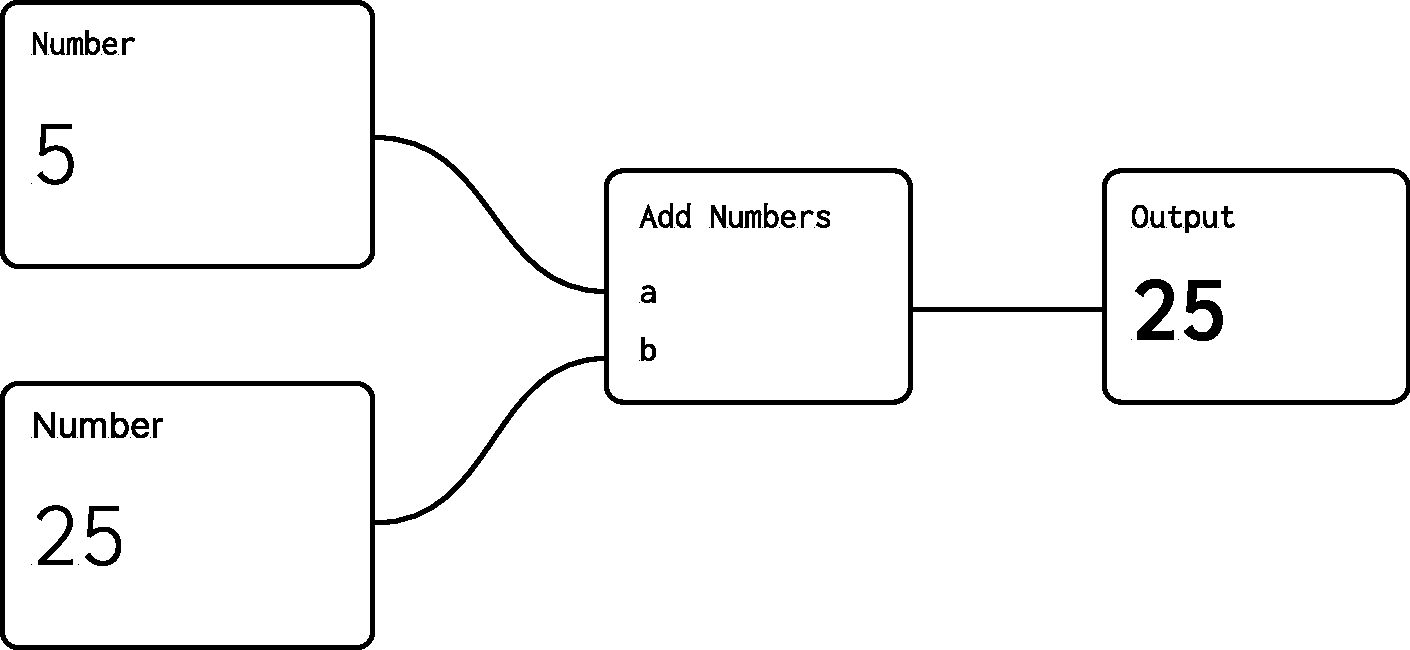
\includegraphics[width=\textwidth]{ideas/nodes.pdf}
\caption{Illustration eines Node-Systems}
\end{figure}
\linebreak
\linebreak
WebAssembly bietet sich hier gut an, da es plattformunabhängig, isoliert und performant ist \cite{Haas2017}. Gerade die Isolation der einzelnen Module ist spannend, da sie es möglich macht Nodes von unterschiedlichen Quellen zu laden, und trotzdem die Sicherheit des Hostsystems zu gewährleisten.
\linebreak
\linebreak
Dies wiederum würde es erlauben, ein generelles Framework bereitzustellen, bei denen node-basierte UI's für unterschiedliche Anwendungsfälle und dank der cross-plattform Eigenschaften von WebAssembly auch für unterschiedliche Plattformen erstellt werden können.
\linebreak
\linebreak
Die Implementierung wird im Kontext einer \href{https://plant.max-richter.dev}{3D-Anwendung} stattfinden, da ich in diesem Bereich viel Erfahrung habe. Außerdem werden in dieser speziellen Anwendung große Datenmengen zwischen den Nodes hin- und hertransportiert, was die Performance-Problematik gut verdeutlichen sollte.

\subsection{Anwendungsgebiete}
Node-basierte visuelle Programmiersprachen werden in unterschiedlichsten Anwendungsfällen eingesetzt. Darunter fallen unter anderem 3D Modellierung \cite{houdini}, Datenverarbeitung \cite{rapidminer}, Bild- und Videobearbeitung \cite{davinci}, IoT \cite{nodered} und viele mehr. 
\linebreak
\linebreak
In meinem eigenen Tool \href{https://plant.max-richter.dev}{Plantarium} habe ich eine node-basierte visuelle Programmiersprache implementiert, die es Nutzer*innen ermöglicht, parametrische 3D Pflanzen zu erstellen. Des Weiteren könnte man eine interaktive Lernumgebung für Kinder entwickeln, bei der sie spielerisch die Grundlagen der Programmierung erlernen können.

\section{Abgeleitete Forschungsfrage}
Inwieweit eignet sich WebAssembly als Grundlage für eine node-basierte visuelle Programmiersprache?  
\linebreak
\linebreak
Welche Auswirkungen haben die spezifischen Vor- und Nachteile von WebAssembly auf die Realisierbarkeit, Funktionalität, Nutzerfreundlichkeit, Performance, Flexibilität und Robustheit einer solchen Programmiersprache?

\section{Vorgehen}
\subsection{Literatur Recherche}
Als Erstes werde ich eine allgemeine Literaturrecherche zu den Themen \topic{WebAssembly}, \topic{visuelle Programmiersprachen} und im speziellen \topic{node-basierte visuelle Programmiersprachen} durchführen.

\subsection{Recherche von bestehenden Lösungen}
Es existieren bereits einige node-basierte visuelle Programmiersprachen mit unterschiedlichen Ansätzen. Diese werde ich umfassend recherchieren und spezifisch auf die Punkte untersuchen, die ich in meiner Anforderungsanalyse festgelegt habe.

\subsection{Anforderungsanalyse}
Nun werde ich festlegen, welche Anforderung meine Implementierung erfüllen sollte. Hierbei werde ich meine potenzielle Nutzergruppe definieren und ausgehend von dieser funktionale Anforderungen wie zum Beispiel das Herunterladen von Nodes und nicht-funktionale Anforderungen wie zum Beispiel Performance, Skalierbarkeit und Sicherheit definieren.

\subsection{Implementierung}
Der Großteil der Arbeit wird in der Implementierung liegen. Hierbei sehe ich im Moment zwei Bereiche, die besonders interessant sind. Zum einen die Performance, da die Kommunikation zwischen einzelnen Nodes höchstwahrscheinlich über das Hostsystem laufen muss. Zweitens muss man eine Möglichkeit finden wie die einzelnen Nodes angeben welche Inputs sie erwarten. 

\subsection{Evaluation}
Im letzten Schritt werde ich untersuchen, inwieweit meine Implementierung die Punkte in meiner Anforderungsanalyse erfüllt. Der Fokus hierbei wird auf der vom User wahrgenommenen Latenz liegen, da dies ein wichtiger Faktor für eine gute User-Experience ist. \cite{6876022}

\section{Formales}
Geplantes Startdatum: 10.02.2024
\linebreak
Sperrvermerk geplant: nein
\linebreak
Begründung: n.z.

\section{Externer Kooperationspartner}
n.z.

\pagebreak

\printbibliography

\end{document}
